%%%%%%%%%%%%%%%%%%%%%%%%%%%%%%%%%%%%%%%%%%%%%%%%%%%%%%%%%%%%%%%%%%%%%%%%%%%%%%%%%%%%%%%%%%%%%%%%%%%%
\gls{SNMP} es un protocolo de capa de aplicación usado para la recolección y organización de
información de los dispositivos gestionados y la modificación de dicha información con el fin de 
modificar el comportamiento de dichos dispositivos. Entre los dispositivos que soportan SNMP 
encontramos módems, router, switches, servidores, estaciones de trabajo, etc.

La base de \gls{SNMP} es un simple conjunto de operaciones que permite a los administradores cambiar el
estado de dispositivos SNMP. Por ejemplo, se puede usar \gls{SNMP} para apagar una interfaz de un router o
comprobar la velocidad a la que una interfaz Ethernet está operando. 

\subsubsection{Gestores y Agentes}

En el mundo \gls{SNMP} existen dos tipos de entidades: gestores (\gls{SNMP} Managers) y agentes. 

%%%%%%%%%%%%%%%%%%%%%%%%%%%%%%%%%%%%%%%%%%%%%%%%%%%%%%%%%%%%%%%%%%%%%%%%%%%%%%%%%%%%%%%%%%%%%%%%%%%%
Un \textbf{SNMP Manager} también llamado Sistema de Gestión de Red (Network Management System o NMS)
es una entidad responsable de la comunicación con los agentes SNMP disponible en la red. Típicamente
es un servidor que ejecuta uno o varios sistemas de gestión de red. Sus principales tareas son:

\begin{itemize}
    \item Consultar a los agentes
    \item Obtener las respuestas enviadas por los agentes
    \item Establecer o cambiar valores de variables en los agentes
    \item Recibir notificaciones eventos de los agentes de forma asíncrona
\end{itemize}

Los agentes SNMP con programas que recolectan información local de los dispositivos en los que están
instalador y la hacen disponible para los SNMP Managers. Las funciones de un agente SNMP son las
siguientes:

\begin{itemize}
    \item Recolectar información acerca de su entorno local
    \item Almacenar y devolver la información definida en sus bases de datos.
    \item Enviar señales a los gestores cuando ocurre un evento
    \item Actuar como un proxy para los nodos no gestionables mediante SNMP
\end{itemize}

En la Figura \ref{fig:diagrama_comunicaciones_snmp} podemos observar como se organizan estas dos
entidades. 

\begin{figure}[ht]
    \centering
    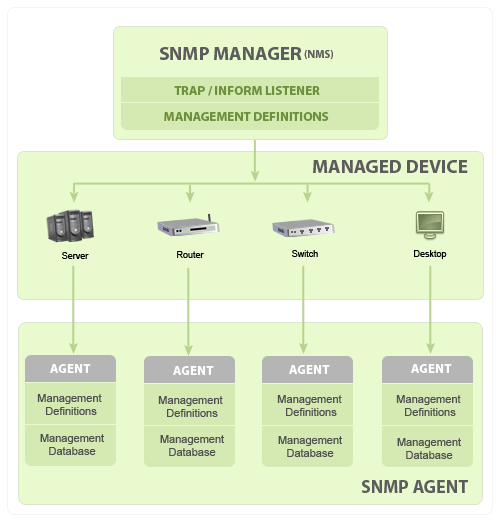
\includegraphics[width=10cm]{graphics/snmp-components}
    \caption{Diagrama básico de comunicaciones SNMP}
    \label{fig:diagrama_comunicaciones_snmp}
\end{figure}

%%%%%%%%%%%%%%%%%%%%%%%%%%%%%%%%%%%%%%%%%%%%%%%%%%%%%%%%%%%%%%%%%%%%%%%%%%%%%%%%%%%%%%%%%%%%%%%%%%%%
\subsubsection{\gls{MIB}}
La Base de Información Gestionada (\gls{MIB}) es un tipo de base de datos que contiene información
jerárquica, con estructura de árbol, de los parámetros gestionables de cada dispositivo SNMP. La
jerarquía MIB se organiza en distintos niveles que se asignan a distintas organizaciones. Los 
primeros niveles están asignados a organizaciones de normalización (ISO, CCITT, etc) mientras que 
los niveles más bajos están asignadas a organizaciones asociadas. En la Figura \ref{fig:mib_tree} 
se puede observas esta forma de organización.


Existe un gran número de MIBs definidos por organizaciones como la \gls{IETF} así como entidades
privadas y fabricantes. La base de datos más común para la gestión de equipos en Internet es la base
MIB-II definida en el \textit{RFC1213} y ampliada con la aparición de las versiones 2 y 3 de SNMP. 
Este MIB es muy importante porque es obligatorio para todos los agentes SNMP de internet y contiene
información acerca del sistema, interfaces así como aspectos de IP (incluidas las tablas de
enrutamiento).


Todos los objetos tienen un identificador único denominado OID que permiten la identificación numérica
de cualquier nodo. Por ejemplo, sirviéndonos de la Figura \ref{fig:mib_tree} podemos ver que el del
objeto \textit{iso.org.dod.internet.mgmt.mib-2.system.sysDescr} tiene el OID 1.3.6.1.2.1.1.1.

\begin{figure}[ht]
    \centering
    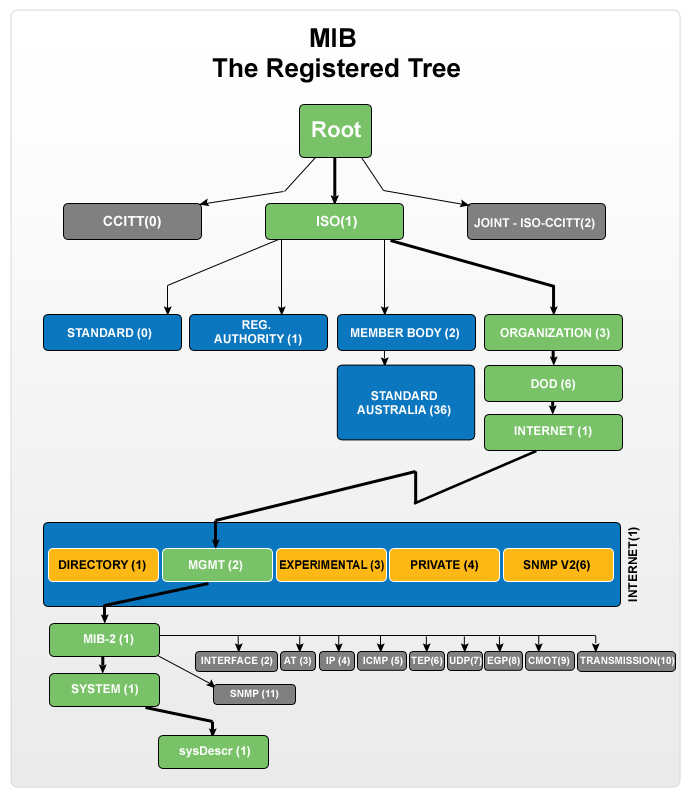
\includegraphics[width=10cm]{graphics/mib-oid-tree}
    \caption{Árbol MIB (parcial)}
    \label{fig:mib_tree}
\end{figure}

%%%%%%%%%%%%%%%%%%%%%%%%%%%%%%%%%%%%%%%%%%%%%%%%%%%%%%%%%%%%%%%%%%%%%%%%%%%%%%%%%%%%%%%%%%%%%%%%%%%%
\subsubsection{Operaciones básicas de SNMP}

Las operaciones que pueden realizar dentro del protocolo SNMP son las siguientes
\cite{mauro2005essential}:

\begin{itemize}
    \item GET: La operación GET es una petición enviada por un gestor a un agente para obtener uno o
    más valores del agente. Figura \ref{fig:snmp_get}
    \item GET NEXT: Esta operación es similar a GET. La principal diferencia es que GET NEXT obtiene
    el valor del siguiente OID del árbol MIB.
    \item GET BULK (SNMPv2 y v3): Operación usada para obtener grandes volúmenes de datos desde tablas
    MIB grandes.Figura \ref{fig:snmp_bulk}
    \item SET: Esta operación es usada por los gestores para modificar o asignar un valor dentro de un
    agente.Figura \ref{fig:snmp_set}
    \item TRAPS: Los TRAPS son señales enviadas por los agentes para notificar a los gestores de algún
    evento.Figura \ref{fig:snmp_trap}
    \item INFORM: similar a una TRAP, pero a diferencia de este INFORM incluye la confirmación por
    parte del gestor \gls{SNMP} de la recepción del mensaje
    \item RESPONSE: este es el comando usado para devolver valores a los gestores SNMP.
\end{itemize}

\begin{figure}
    \centering
    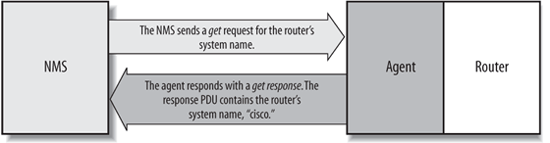
\includegraphics[width=.5\linewidth]{graphics/snmp_get}
    \caption{SNMP Get Sequence}
    \label{fig:snmp_get}
\end{figure}

\begin{figure}
    \centering
    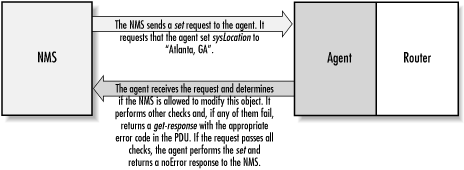
\includegraphics[width=.5\linewidth]{graphics/snmp_set}
    \caption{SNMP Set Sequence}
    \label{fig:snmp_set}
\end{figure}

\begin{figure}
    \centering
    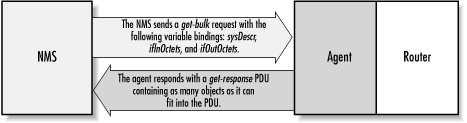
\includegraphics[width=.5\linewidth]{graphics/snmp_get_bulk}
    \caption{SNMP Get Bulk Sequence}
    \label{fig:snmp_bulk}
\end{figure}

\begin{figure}
    \centering
    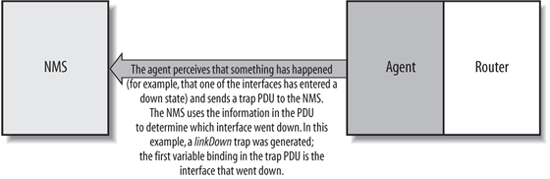
\includegraphics[width=.5\linewidth]{graphics/snmp_trap}
    \caption{SNMP Trap Sequence}
    \label{fig:snmp_trap}
\end{figure}